%%% License: Creative Commons Attribution Share Alike 4.0 (see https://creativecommons.org/licenses/by-sa/4.0/)
%%% Slides are based heavily on earlier versions of this course taught by Jesper Rudiger.

\documentclass[english,10pt]{beamer}
\DeclareGraphicsExtensions{.eps, .pdf,.png,.jpg,.mps,}
\usetheme{reMedian}
\usepackage{parskip}
\makeatother

\renewcommand{\baselinestretch}{1.2} 

\usepackage{amsmath, amssymb, amsfonts, amsthm}
\usepackage{enumerate}
\usepackage{hyperref}
\usepackage{url}
\usepackage{bbm}
\usepackage{color}

\usepackage{tikz}
\usepackage{tikzscale}
\newcommand*\circled[1]{\tikz[baseline=(char.base)]{
\node[shape=circle,draw, inner sep=-20pt] (char) {#1};}}
\usetikzlibrary{automata,positioning}
\usetikzlibrary{decorations.pathreplacing}
\usepackage{pgfplots}
\usepgfplotslibrary{fillbetween}
\usepackage{graphicx}

\usepackage{setspace}
\thinmuskip=1mu
\medmuskip=1mu 
\thickmuskip=1mu 

\theoremstyle{definition} 
\newtheorem{thm}{Theorem}
\newtheorem{claim}{Claim}
\newtheorem{proposition}{Proposition}
\usecolortheme{default}
\usepackage{verbatim}
\usepackage[normalem]{ulem}
\usepackage{appendixnumberbeamer}


%\usepackage[export]{adjustbox}[2011/08/13]
%\usepackage[round]{natbib}
%\usepackage{multicol}
%\usepackage{mathrsfs}
%\usepackage{epsfig}
%\usepackage{epstopdf}
%\usepackage{subfigure}
%\usepackage{indentfirst}
%\usepackage{float}
%\usepackage{multirow} % multirow cells in tables



\title{Financial Markets Microstructure \\ Lecture 1}

\subtitle{Introduction and institutions \\
Chapters 0 and 1 of FPR}

\author{Egor Starkov}

\date{K{\o}benhavns Unversitet \\
	Spring 2020}



\begin{document}
\frame[plain]{\titlepage}
\addtocounter{framenumber}{-1}



\section{Practicalities}

\begin{frame}{Today's plan}
\tableofcontents[]
\end{frame}


\begin{frame}{Contact Information}
Lecturer: Egor Starkov
\begin{itemize}
	\item Email: \href{mailto:egor.starkov@econ.ku.dk}{\texttt{egor.starkov@econ.ku.dk}}
	\item Office: 26.1.13
	\item Office hours: by appointment
\end{itemize}
\end{frame}


\begin{frame}{Course Information}
\begin{itemize}
	\item 2 hours of lectures once or twice a week
	\item \alert{Lectures}: Wednesdays 13.00-15.00, CSS 35-01-05 (week 6-21); 
		\\ \structure{Sections}: Fridays 10.00-12.00, CSS 25-01-53 (weeks 7,9,11,13,17).
	\item Everything (lectures, problem sets for exercise classes, etc.) is on Absalon -- check regularly or subscribe for updates.
	\item I will upload the slides before the lectures for you to print out.
\end{itemize}
\end{frame}


\begin{frame}{Problem sets and Exam}
\begin{itemize}
	\item Will give exercises after lectures (esp. in earlier part of the course).
	\begin{itemize}
		\item These are voluntary. We will solve them in sections
	\end{itemize}
	\item Will assign 2 problem sets (larger, cumulative, more open-ended).
	\begin{itemize}
		\item Voluntary too. Take them as an opportunity to check your progress
	\end{itemize}
	\item The final exam will be a 12-hours take-home exam.
\end{itemize}
\end{frame}


\begin{frame}{Course Materials}
\begin{itemize}
	\item We will be following the textbook for the most part (exercises included),
	\begin{itemize}
		\item Thierry Foucault, Marco Pagano and Ailsa R{\"o}ell: “Market Liquidity: Theory Evidence and Policy,” Oxford University Press, 2013. 439 pages.
	\end{itemize}
	\item Switch to research articles towards the end of the course.
\end{itemize}
\end{frame}




\section{Introduction}

\begin{frame}{Today's plan}
\tableofcontents[currentsection]
\end{frame}


\begin{frame}{Today's plan}
\begin{itemize}
	\item Get a grasp of what we mean, broadly speaking, when we talk about financial markets
	\item Motivate why we want to study financial markets, and why they are different from the markets you have seen until now
	\item Introduce some of the key concepts and language
	\item Look at some basic examples of how markets work
	\item Categorize the most important types of institutions
	\item Think about what policy issues might be relevant
\end{itemize}
\end{frame}


\begin{frame}{Motivating questions}
\begin{itemize}
	\item How are market prices created? How are they influenced by traders?
	\item How should traders act on their information?
	\item Do the market rules matter? And which rules are good for whom?
	\item How do we measure if markets are working well?
	\begin{itemize}
		\item Liquidity/depth (a lot more on that later)
		\item Volume
		\item Efficiency
		\item Stability
	\end{itemize}
\end{itemize}
%NOTE: talk here about how this course departs from walrasian markets and dwelves into how it's composed from individual trades
\end{frame}


\begin{frame}{Many things happening now}
\begin{figure}
	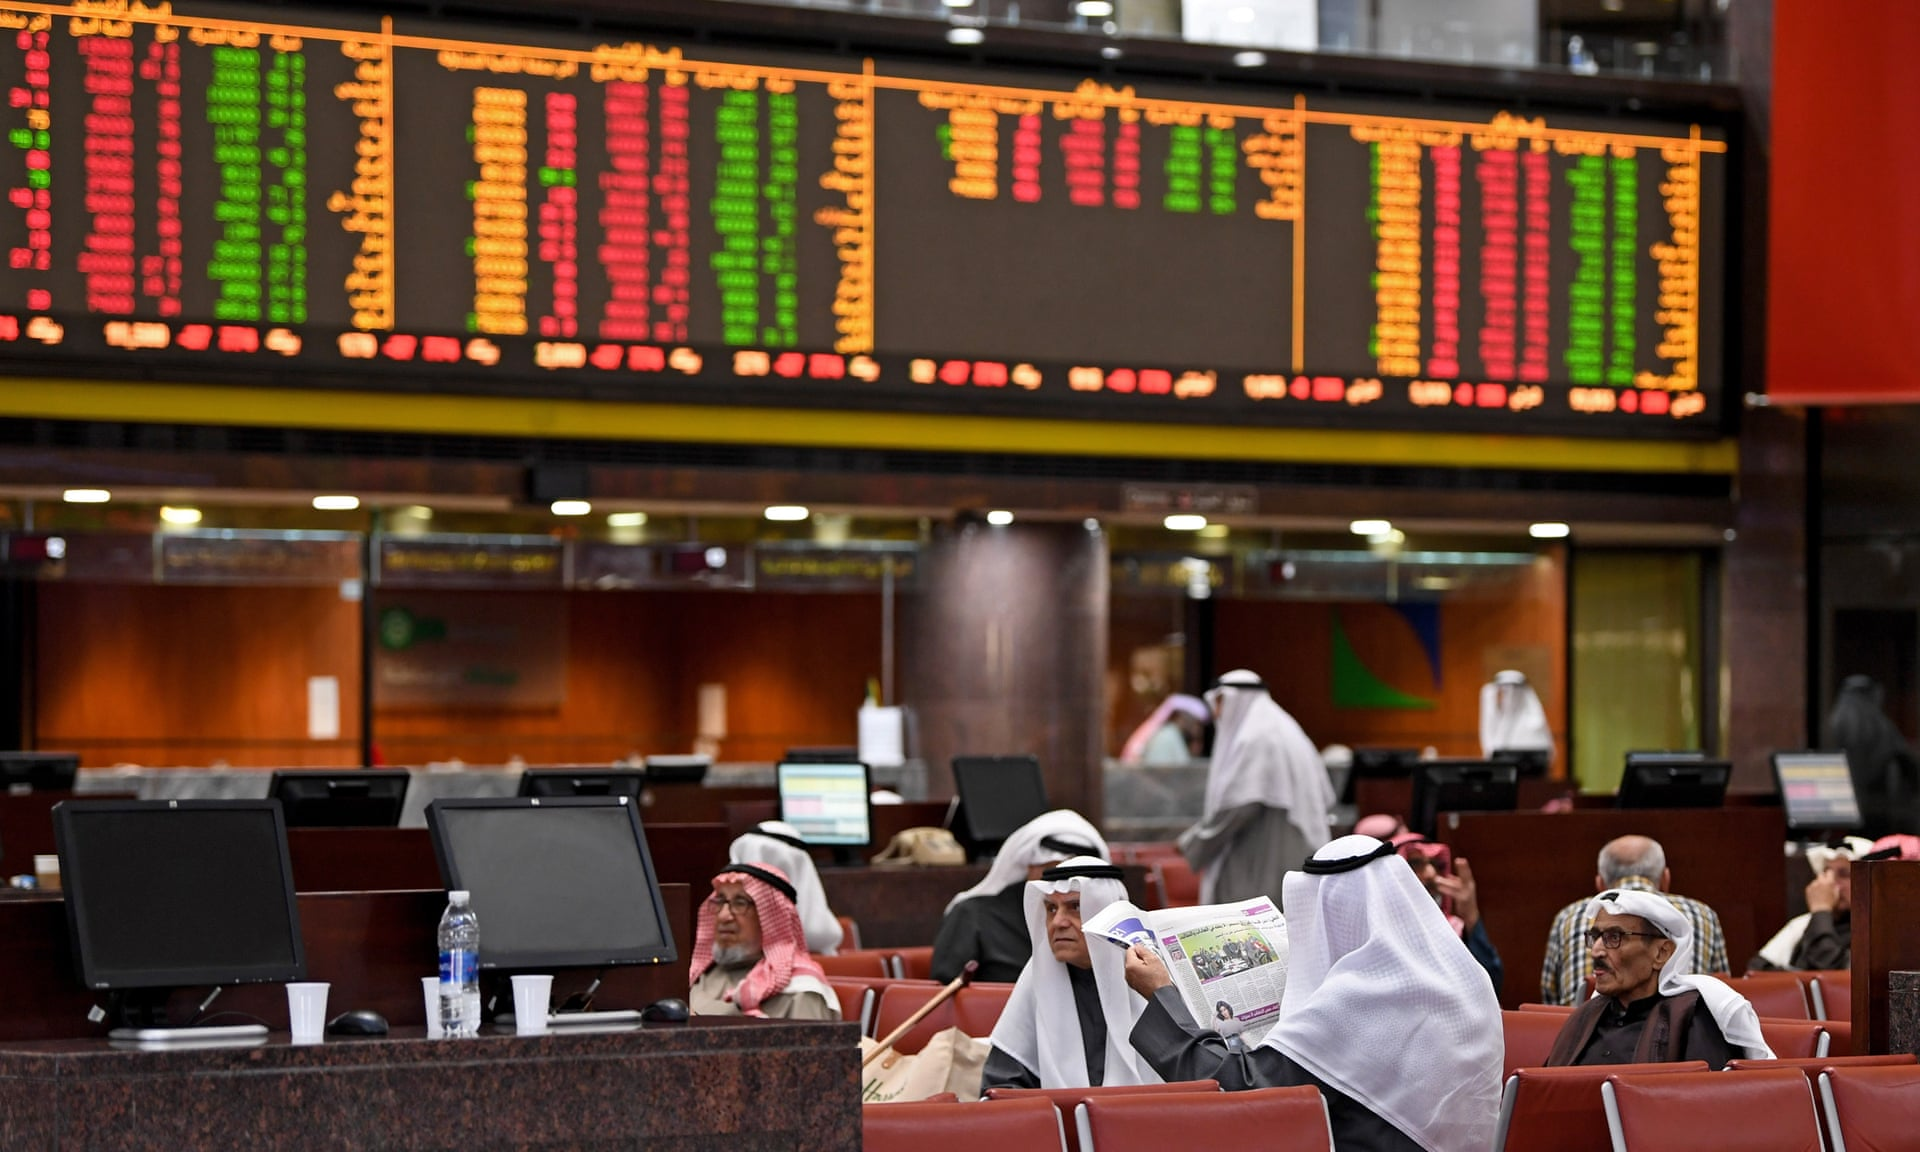
\includegraphics[width=.8\linewidth]{pics/markets2020}
	\caption{The Guardian, January 6}
	%NOTE: photo: Kuwait exchange trading floor.
	%NOTE: Stock exchanges dropped on Jan 7 after Trump's attack on Iran and the retaliation that followed. Oil prices surged. A rebound followed after both sides announced easing out.
\end{figure}
\end{frame}


\begin{frame}{Approach}
\begin{itemize}
	\item Institutional details, policy issues, applications:
	\begin{itemize}
		\item Chapters 1, 6-10; articles
		\item Topics outside book: public information, bubbles
	\end{itemize}
	\item Theories to understand and to analyze policy:
	\begin{itemize}
		\item Chapters 3-4, 6-10; articles
	\end{itemize}
	\item Some empirical issues:
	\begin{itemize}
		\item Chapters 2 and 5; articles
	\end{itemize}
	\item Prerequisites:
	\begin{itemize}
		\item Finance, micro, games, (math)
	\end{itemize}
\end{itemize}
\end{frame}


\begin{frame}{Main goals}
\begin{enumerate}
	\item Explain, discuss and interpret concepts and results from textbook and articles
	\item Derive and analyze results in models
	\item Discuss possible applications of theoretical concepts to problems
\end{enumerate}
Method: Carefully read texts, combine with facts, discuss, try problems
\pause
\quad
\textbf{Disclaimer}: We focus on `rational' models in this course.
Behavioral finance is a complementary and exciting topic. See
Alexander Sebald's course.
\end{frame}


\begin{frame}{Role of Financial Markets}
\begin{itemize}
	\item \textbf{Financial assets}: move wealth across time and contingencies: 
	\begin{itemize}
		\item Financial assets provide `contingent cash flows'
		\item Stocks, bonds, derivatives...
	\end{itemize}
	\item \textbf{Financial markets}: markets for financial assets
	\item Purposes of financial markets:
	\begin{itemize}
		\item Forum for trade in the stock (\alert{consolidation});
		\item Each trader can compare his private valuation against the current price (\alert{transparency});
		\item Guarantee of getting what is paid for (\alert{security})
	\end{itemize}
\end{itemize}
\end{frame}


\begin{frame}{Types of Financial Markets}
\begin{itemize} 
	\item \textbf{Primary markets}: ``Allocate savings to investment''
	\begin{itemize}
		\item Issues of new assets (typically by investment bank)
	\end{itemize}
	\item \textbf{Secondary markets}: ``Reallocate investments over savers''
	\begin{itemize}
		\item Trade in existing assets on exchange
	\end{itemize}	
	\item This course: focus on secondary markets 
\end{itemize}
\end{frame}


\begin{frame}[label=main2]{Trade and Prices}
\begin{itemize}
	\item Price theory is fundamental to economics
	\begin{itemize}
		\item Law of one price; no arbitrage
		%TODO: SMBC here?
	\end{itemize}
	\item In financial markets: often a \textit{bid} and an \textit{ask} price. The difference between the two is called the `bid-ask spread' \hyperlink{bidask}{\beamerbutton{bid-ask}}
	\begin{itemize}
		\item We will spend time analyzing what drives this spread
	\end{itemize}
	\item Important question: How are prices formed?
	\begin{itemize}
		\item Shed light on the invisible hand
		\item Difference to standard market theory: assume that agents are strategic ($\rightarrow$ game theory) 
	\end{itemize}
	\item Do markets result in efficient allocations?
\end{itemize}
\end{frame}


\begin{frame}{Example: Google Stock}
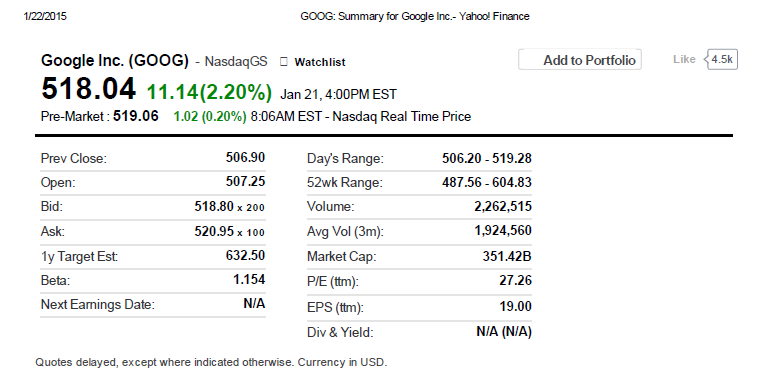
\includegraphics[width=1\linewidth]{pics/StockSummary_Google}
\end{frame}


\begin{frame}[label=main4]{Fundamental Value}
\begin{itemize}
	\item Consider Google Stock
	\item What is the fundamental value of its stock? Where does it come from?
	\begin{enumerate}
		\item R+D
		\item Governance
		\item Marketing
		\item Competition
		\item ...
	\end{enumerate}
	\item In this course: take the `fundamental value' as given and analyze how it translates into prices
	
	\hyperlink{quote}{\beamerbutton{Quote}}
\end{itemize}
\end{frame}


\begin{frame}{Market Liquidity}
\begin{itemize}
	\item So far, you have been used to analyzing (long-run) equilibrium allocations and prices
	\item In practice, prices adjust to temporary imbalances
	\begin{itemize}
		\item Example: too many sellers $\rightarrow$ prices lower in short run
		\item Example: costly to execute large order quickly
	\end{itemize}
	\item These effects are related to the \structure{liquidity} of the asset
	\begin{itemize}
		\item Wikipedia: `market liquidity' is a market's ability to facilitate an asset being sold quickly without having to reduce its price very much
		\item Easy to sell a Google stock (many potential buyers), but maybe hard for a stock of a small Danish company
	\end{itemize}
	\item We will develop measures of liquidity in this course
	\item More liquid assets may be more valuable
\end{itemize}
\end{frame}


\begin{frame}{Market depth}
\begin{itemize}
	\item Prices are not always immediately available, even at an exchange
	\begin{itemize}
		\item You may observe previous trading prices, but nothing assures that future trading prices will be the same
		\item You may observe quotes from sellers/buyers, but quotes are normally only valid for a specific amount of stocks
	\end{itemize}
	\item A useful concept is \structure{market depth}: it measures how big an order is required to change the price of an asset by, say, 10 cents
\end{itemize}
\end{frame}


\begin{frame}{Finally... The Big Issue}
\begin{itemize}
	\item Since this is a course on financial markets, we will also try to speak (a bit) about recent big events.
	For instance...
	
	\begin{minipage}{.4\textwidth}
		\begin{figure}
		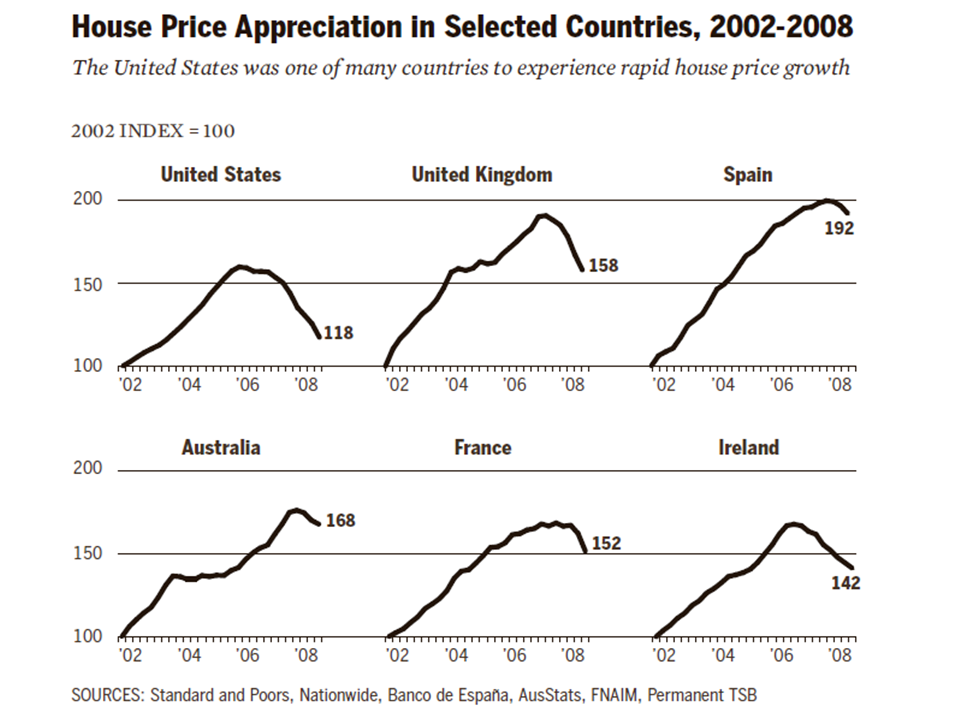
\includegraphics[width=1\linewidth]{pics/Graph_HousePrices}
		\caption{Housing bubble}
		\end{figure}
	\end{minipage}
	\quad
	\begin{minipage}{.4\textwidth}
		\begin{figure}
		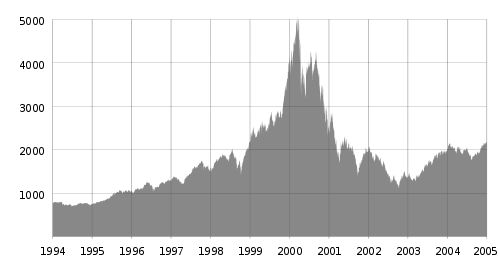
\includegraphics[width=1.3\linewidth]{pics/Graph_Nasdaq}
		\caption{Tech bubble (Nasdaq index)}
		\end{figure}
	\end{minipage}
	\item The last lectures of the course will be about this
\end{itemize}
\end{frame}



\section{Institutions}

\begin{frame}{Today's plan}
\tableofcontents[currentsection]
\end{frame}


%\begin{frame}{Asset Markets}
%\begin{itemize}
%	%TODO: cut this slide?
%	\item \textbf{Markets}: facilitate trade between investors and savers
%	\item \textbf{Speculators}: interact with markets
%	\item \textbf{Intermediation}: done by dealers/brokers or automated systems
%	\item \textbf{Matching}: thus, the market matches buyers with sellers - important to attract both types of traders
%\end{itemize}
%\end{frame}


\begin{frame}{Market Setups}
Two rough categories of market setups
\begin{itemize}
	\item (i) Order-driven markets
	\begin{itemize}
		\item Continuous
		\item Call
	\end{itemize}
	\item (ii) Dealer markets
\end{itemize}
\end{frame}


\begin{frame}{Order types}
\begin{itemize}
	\item There's a tremendous amount of different order types: we focus on 'limit orders' and 'market orders'
	\item \textbf{Limit order}. Specify a quantity and a price. E.g. ``will buy 500 shares at below price 40''
	\item \textbf{Market order}. Specify quantity; to execute immediately at best available price
	\item Relation to liquidity:
	\begin{itemize}
		\item Patient traders are more passive: use limit orders (provide liquidity)
		\item Impatient traders are more aggressive: use market orders (take liquidity)
	\end{itemize}
\end{itemize}
\end{frame}


\begin{frame}{Order-driven markets}
\begin{itemize}
	\item Timing
	\begin{enumerate}
		\item Orders are submitted
		\item Trades are arranged
	\end{enumerate}
	\item The markets can vary in different ways
	\begin{itemize}
		\item Frequency of trading: how often?
		\item Order precedence: price/time/public
		\item Pricing rule: uniform/discriminatory price, determined from orders/taken from other exchange
	\end{itemize}
\end{itemize}
\end{frame}


\begin{frame}{Order-driven markets: Limit order markets}
\begin{itemize}
	\item Some traders post limit orders (provide liquidity)
	\item Some traders post market orders (take liquidity)
	\item Trades occur either through 
	\begin{enumerate}
		\item a limit order 'match' (somebody posts a bid price above the lowest ask price), or
		\item through market orders
	\end{enumerate}
	\item \alert{Discriminatory price}: depends on how your order is matched
	\item Continuous LOB exchanges: NYSE (both electronic and `outcry'), LSE, BATS, Euronext
\end{itemize}
\end{frame}


\begin{frame}[label=main3]{Order-driven markets: Limit order markets}
%TODO: exercise class
Recall this table from the book.
\begin{figure}
	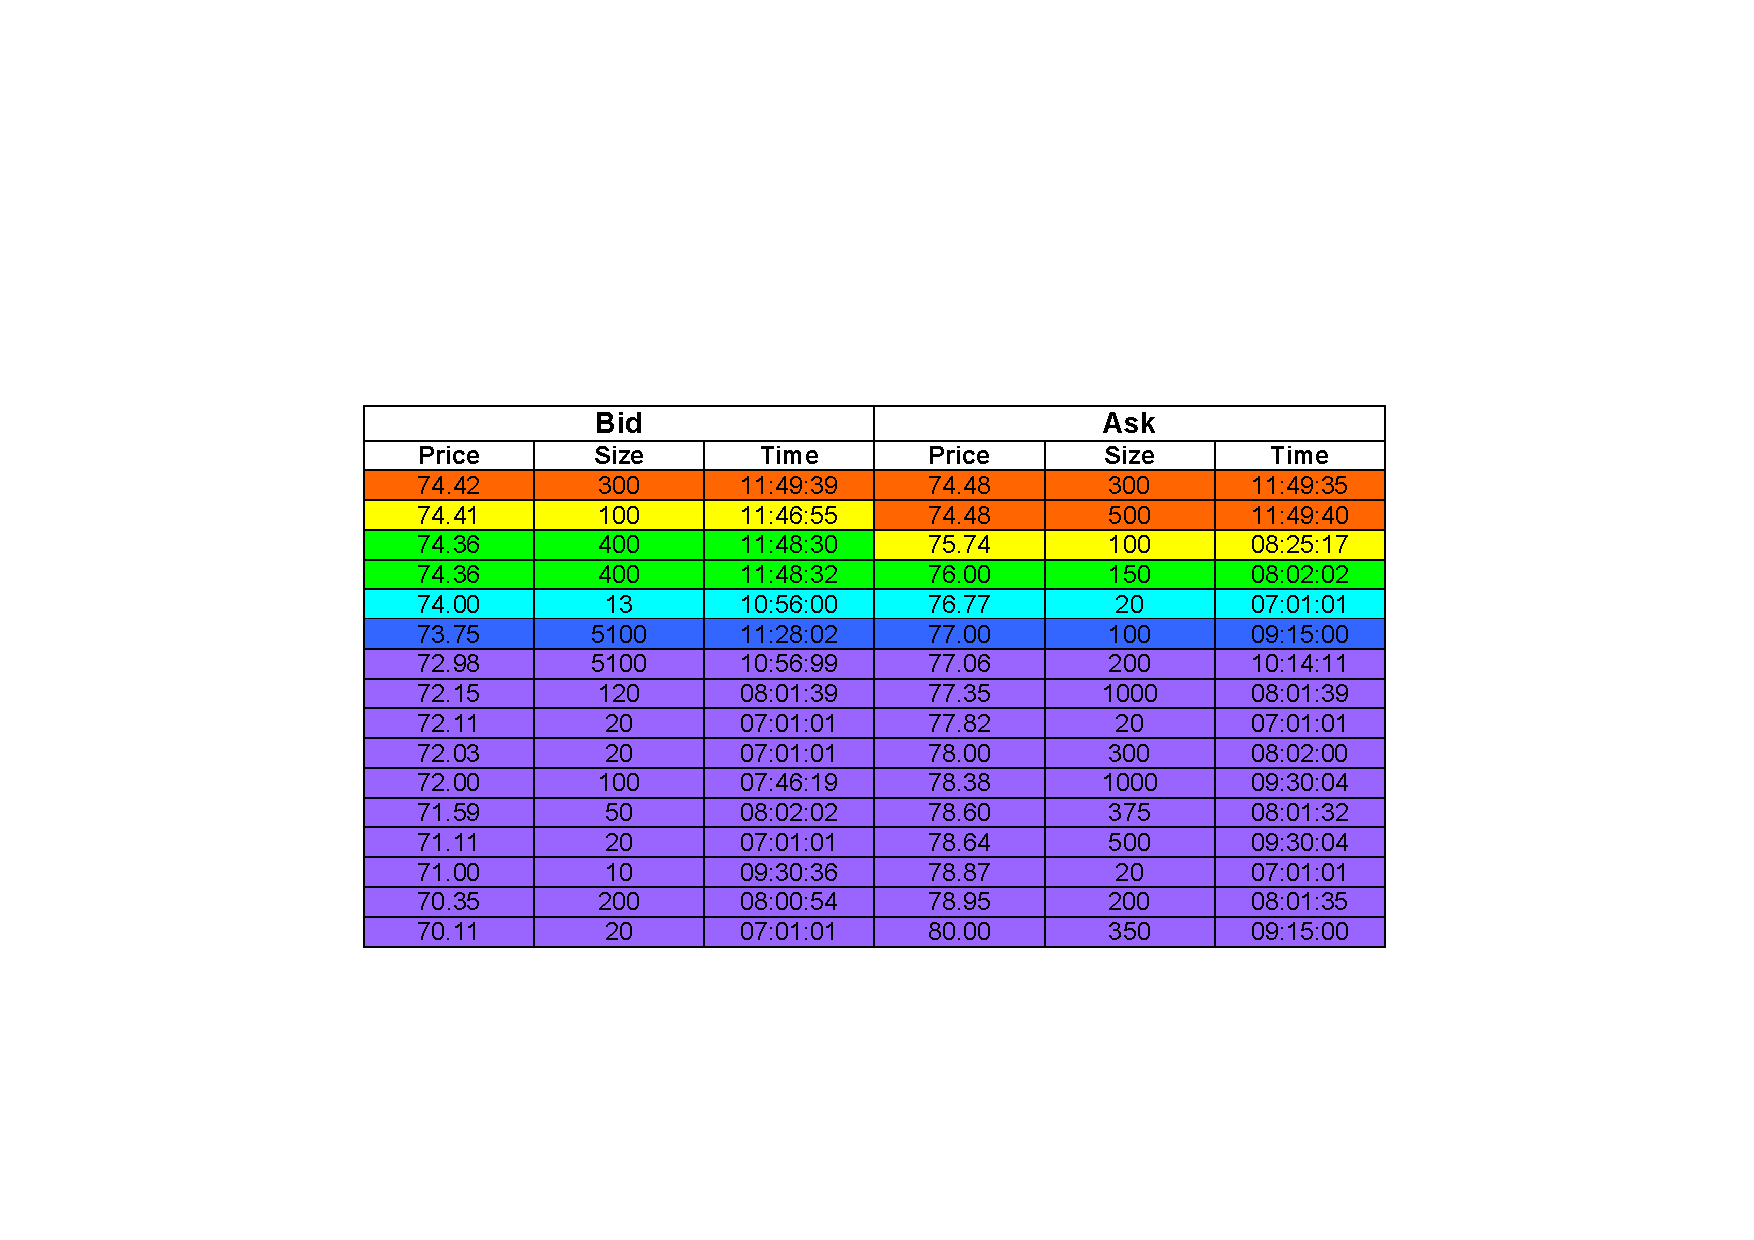
\includegraphics[width=.7\paperwidth]{pics/Image_LOB}
\end{figure}
\hyperlink{LOB}{\beamerbutton{LOB}}
\end{frame}


\begin{frame}{Order-driven markets: Call auctions (batch)}
\begin{itemize}
	\item Orders are collected (in a `batch') and cleared at a certain frequency
	\item The price is chosen so as to maximize the number of executed orders
	\item \textcolor{red}{Uniform price}: all orders in a batch trades at same price
	\item In theory,  very good efficiency properties: all profitable trades are carried out
	\item But... slower than the continuous market
	\item Call auction exchanges: most of the major exchanges (e.g. Nasdaq, LSE, Euronext) operate call auctions together with other trading methods
\end{itemize}
\end{frame}


\begin{frame}{Dealer Markets}
\begin{itemize}
	\item Unlike order-driven markets, prices are fixed by a dealer
	\item He quotes a bid and an ask price (valid up to certain number of shares)
	\item Bid-ask spread:
	\begin{itemize}
		\item Narrow to fend off competitors
		\item Wide to generate trading profits
	\end{itemize}
	\item How competitive are the prices?
	\item Dealer costs:
	\begin{itemize}
		\item Transactions and operations costs
		\item Inventory costs
		\item Adverse selection costs
	\end{itemize}
	\item Dealer exchanges: Nasdaq
\end{itemize}
\end{frame}


\begin{frame}{Exchange versus over-the-counter}
\textbf{Exchange trading}
\begin{itemize}
	\item Organized exchange venues (NYSE, NASDAQ, LSE, ...)
	\item Generally offer a lot of services
	\begin{itemize}
		\item Liquidity and stability through \textit{specialists/market makers}
		\item Clearing and settlement
		\item Transparency
	\end{itemize}
\end{itemize}
\textbf{Over-the-counter (OTC) trading}
\begin{itemize}
	\item Off-exchange venues
	\begin{itemize}
		\item Use quotation systems to match dealers and traders
		\item However, no guarantee of liquidity (no specialists)...
		\item ...nor transparency: may not publish trade information
	\end{itemize}
\end{itemize}
\textbf{Dark liquidity}: Liquidity in `private exchanges' (not public)
%NOTE: Amazon is like an exchange (provides basic products in all categories); eBay/FB is OTC (only matches buyers and sellers);
%NOTE: Difference between OTC and Dark is whether offers/quotes are public or not (although DARK a subset of OTC?)
\end{frame}


\begin{frame}{Comparison}
	What to consider when looking at these markets?
	\begin{itemize}
		\item \textbf{Welfare planner}: Competition - efficiency 
		\item \textbf{Trader}: Liquidity - transparency - information
	\end{itemize}
\end{frame}


\begin{frame}{Regulation}
	Market rules and government regulation:
	
	\textbf{Goals:}
	\begin{itemize}
		\item Protection against insider traders, level the information flow
		\item Stabilize the market, for instance halts and short-sale bans
		\item More generally, select optimal trading structure for each asset type
	\end{itemize}
	\textbf{Methods:}
	\begin{itemize}
		\item Require routing of orders between markets
		\item Transactions tax
		\item Margin requirements
		\item Policies on algorithmic, high-frequent trading
	\end{itemize}
\end{frame}


\begin{frame}{Competition}
\begin{itemize}
	\item Network externalities in trading may favor a single market place (natural monopoly)
	\item Competition may improve the terms offered to traders
	\begin{itemize}
		\item Should regulators require price transparency?
		\item Order routing
		\item Foster competitive market making?
	\end{itemize}
\end{itemize}
\end{frame}


\begin{frame}{Volumes of trade}
\begin{figure}
	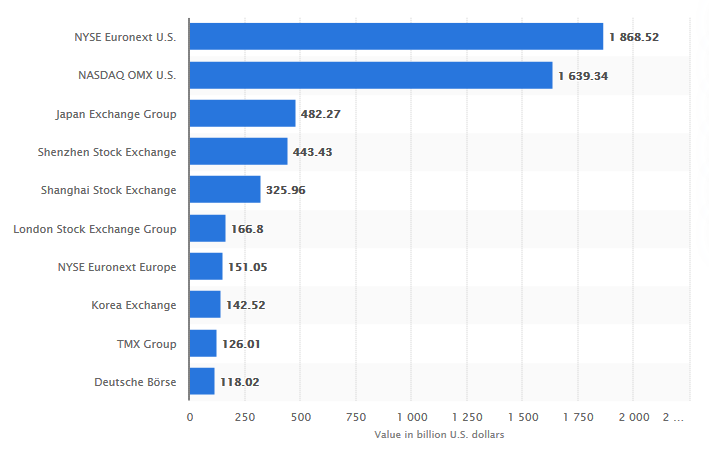
\includegraphics[width=.75\paperwidth]{pics/volumes2018}
\end{figure}
Largest stock exchanges worldwide in 2018, by value of electronic order book share trading, in billion USD (Statista)
\end{frame}


\begin{frame}{Problems for next class}
\begin{itemize}
	%\item In Absalon, I have attached a press release on short selling from the EU Court of Justice, January 22, 2014. Debate the relation among traders, exchanges and regulators, in light of this story.
	\item Find bid and ask prices for Facebook shares and for Microsoft. Which stock exchange do they come from? 
	\item Exercises 1-3 on pages 44-45 in the textbook
\end{itemize}
\end{frame}


\begin{frame}{To finish up: a parable on financial markets (1/4)}
	\centering 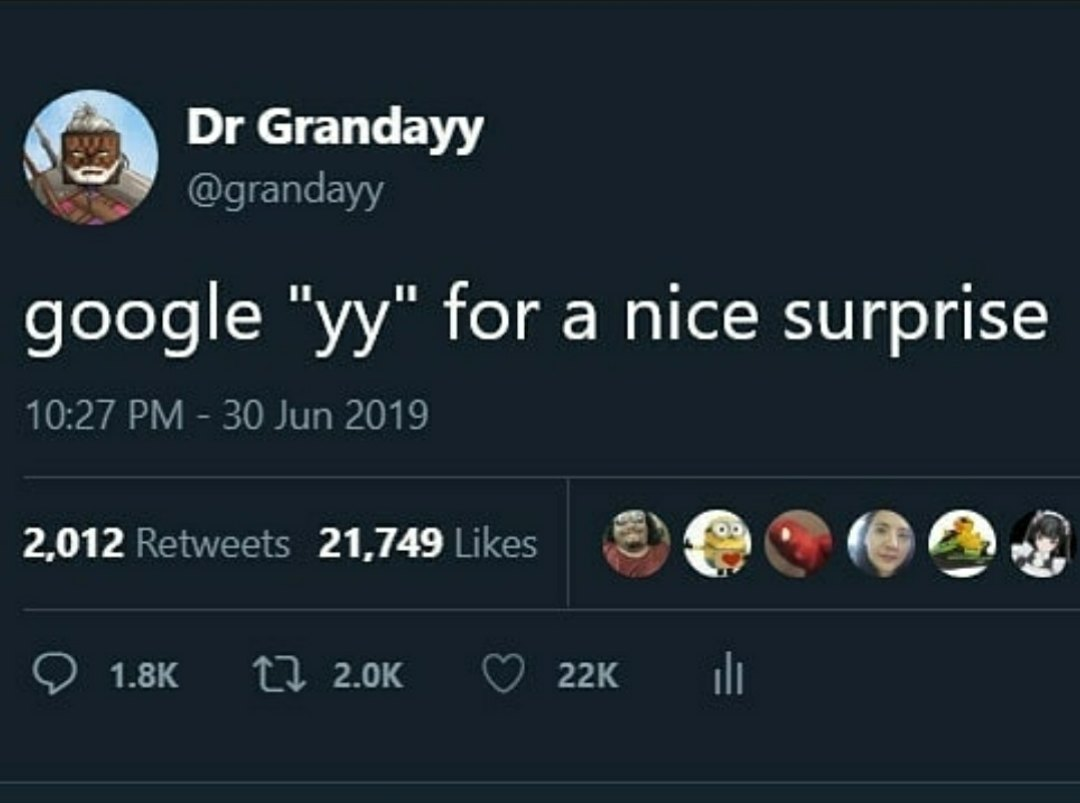
\includegraphics[width=0.6\paperwidth]{pics/yy1}
\end{frame}


\begin{frame}{To finish up: a parable on financial markets (2/4)}
	\centering 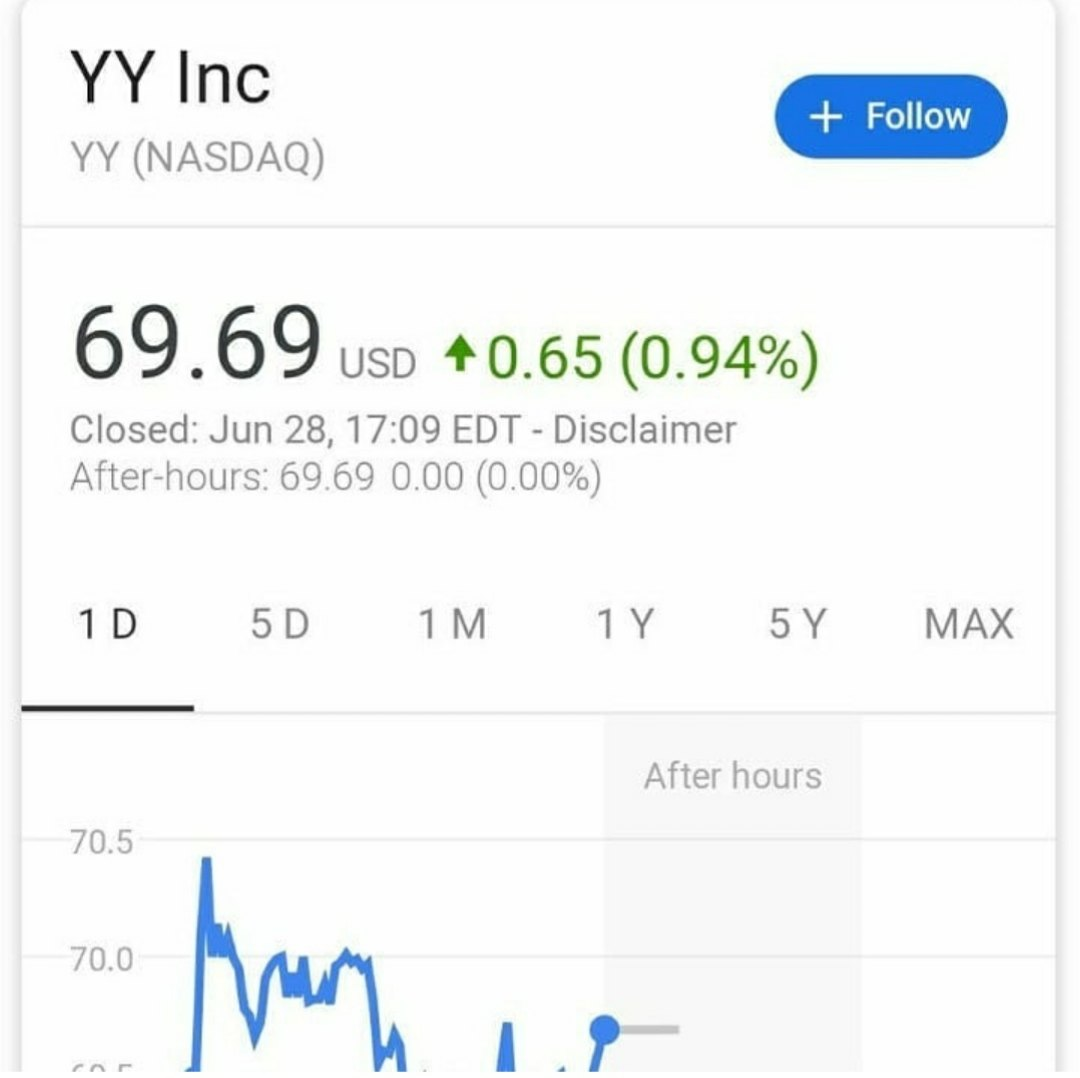
\includegraphics[width=0.6\paperwidth]{pics/yy2}
\end{frame}


\begin{frame}{To finish up: a parable on financial markets (3/4)}
	\centering 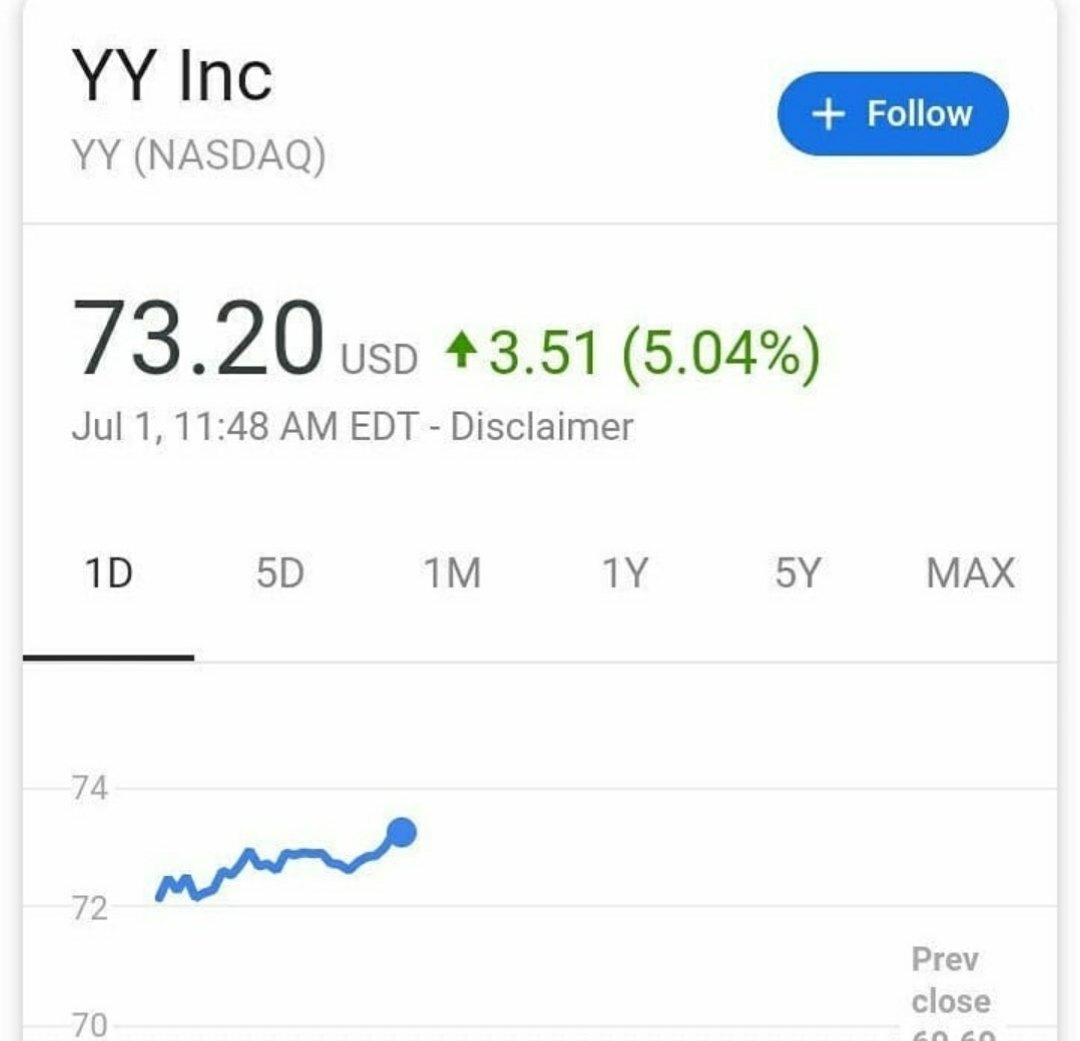
\includegraphics[width=0.6\paperwidth]{pics/yy3}
\end{frame}


\begin{frame}{To finish up: a parable on financial markets (4/4)}
	\centering 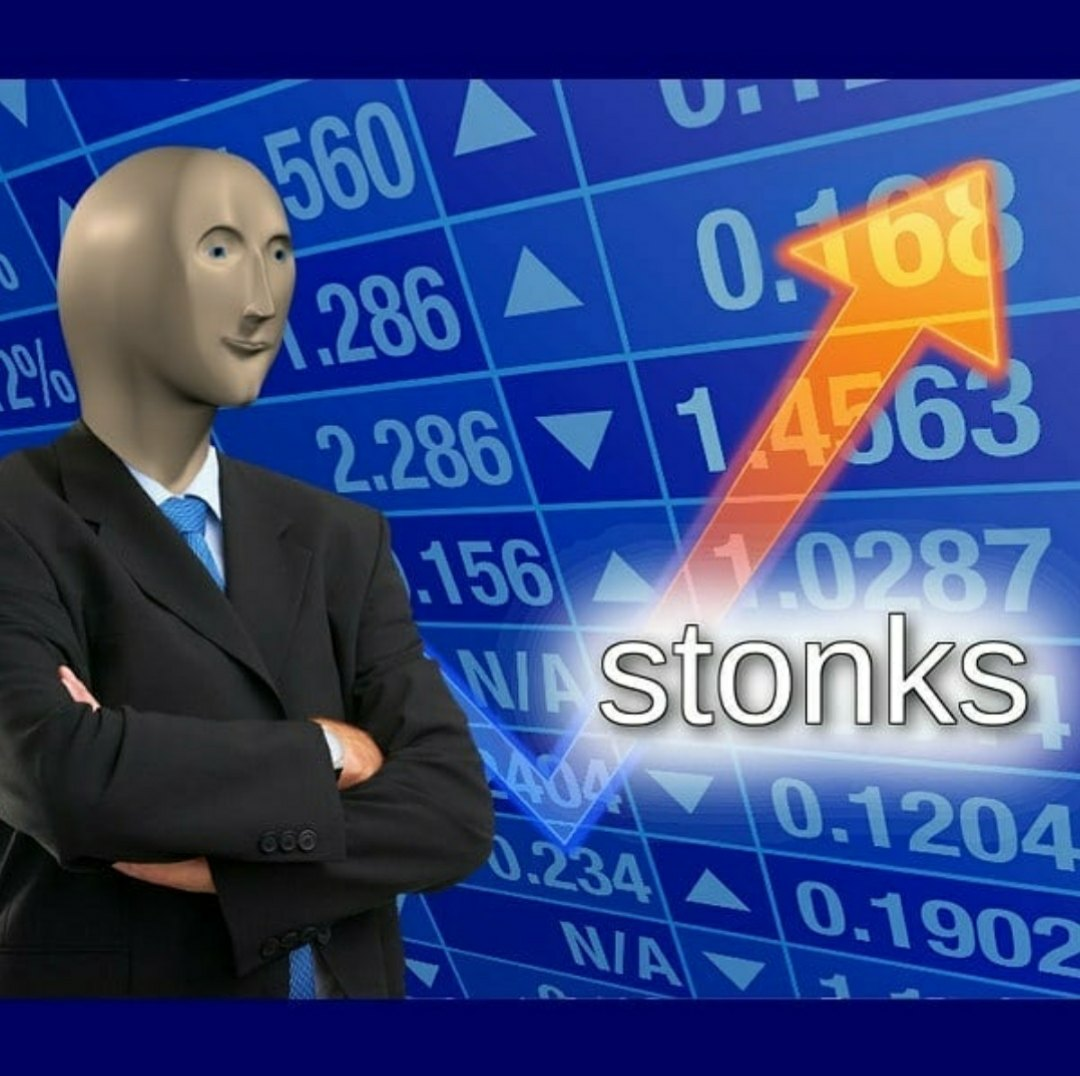
\includegraphics[width=0.6\paperwidth]{pics/yy4}
\end{frame}


\begin{frame}<handout:0>[label=bidask, noframenumbering]{Bid-ask}
	\begin{figure}
	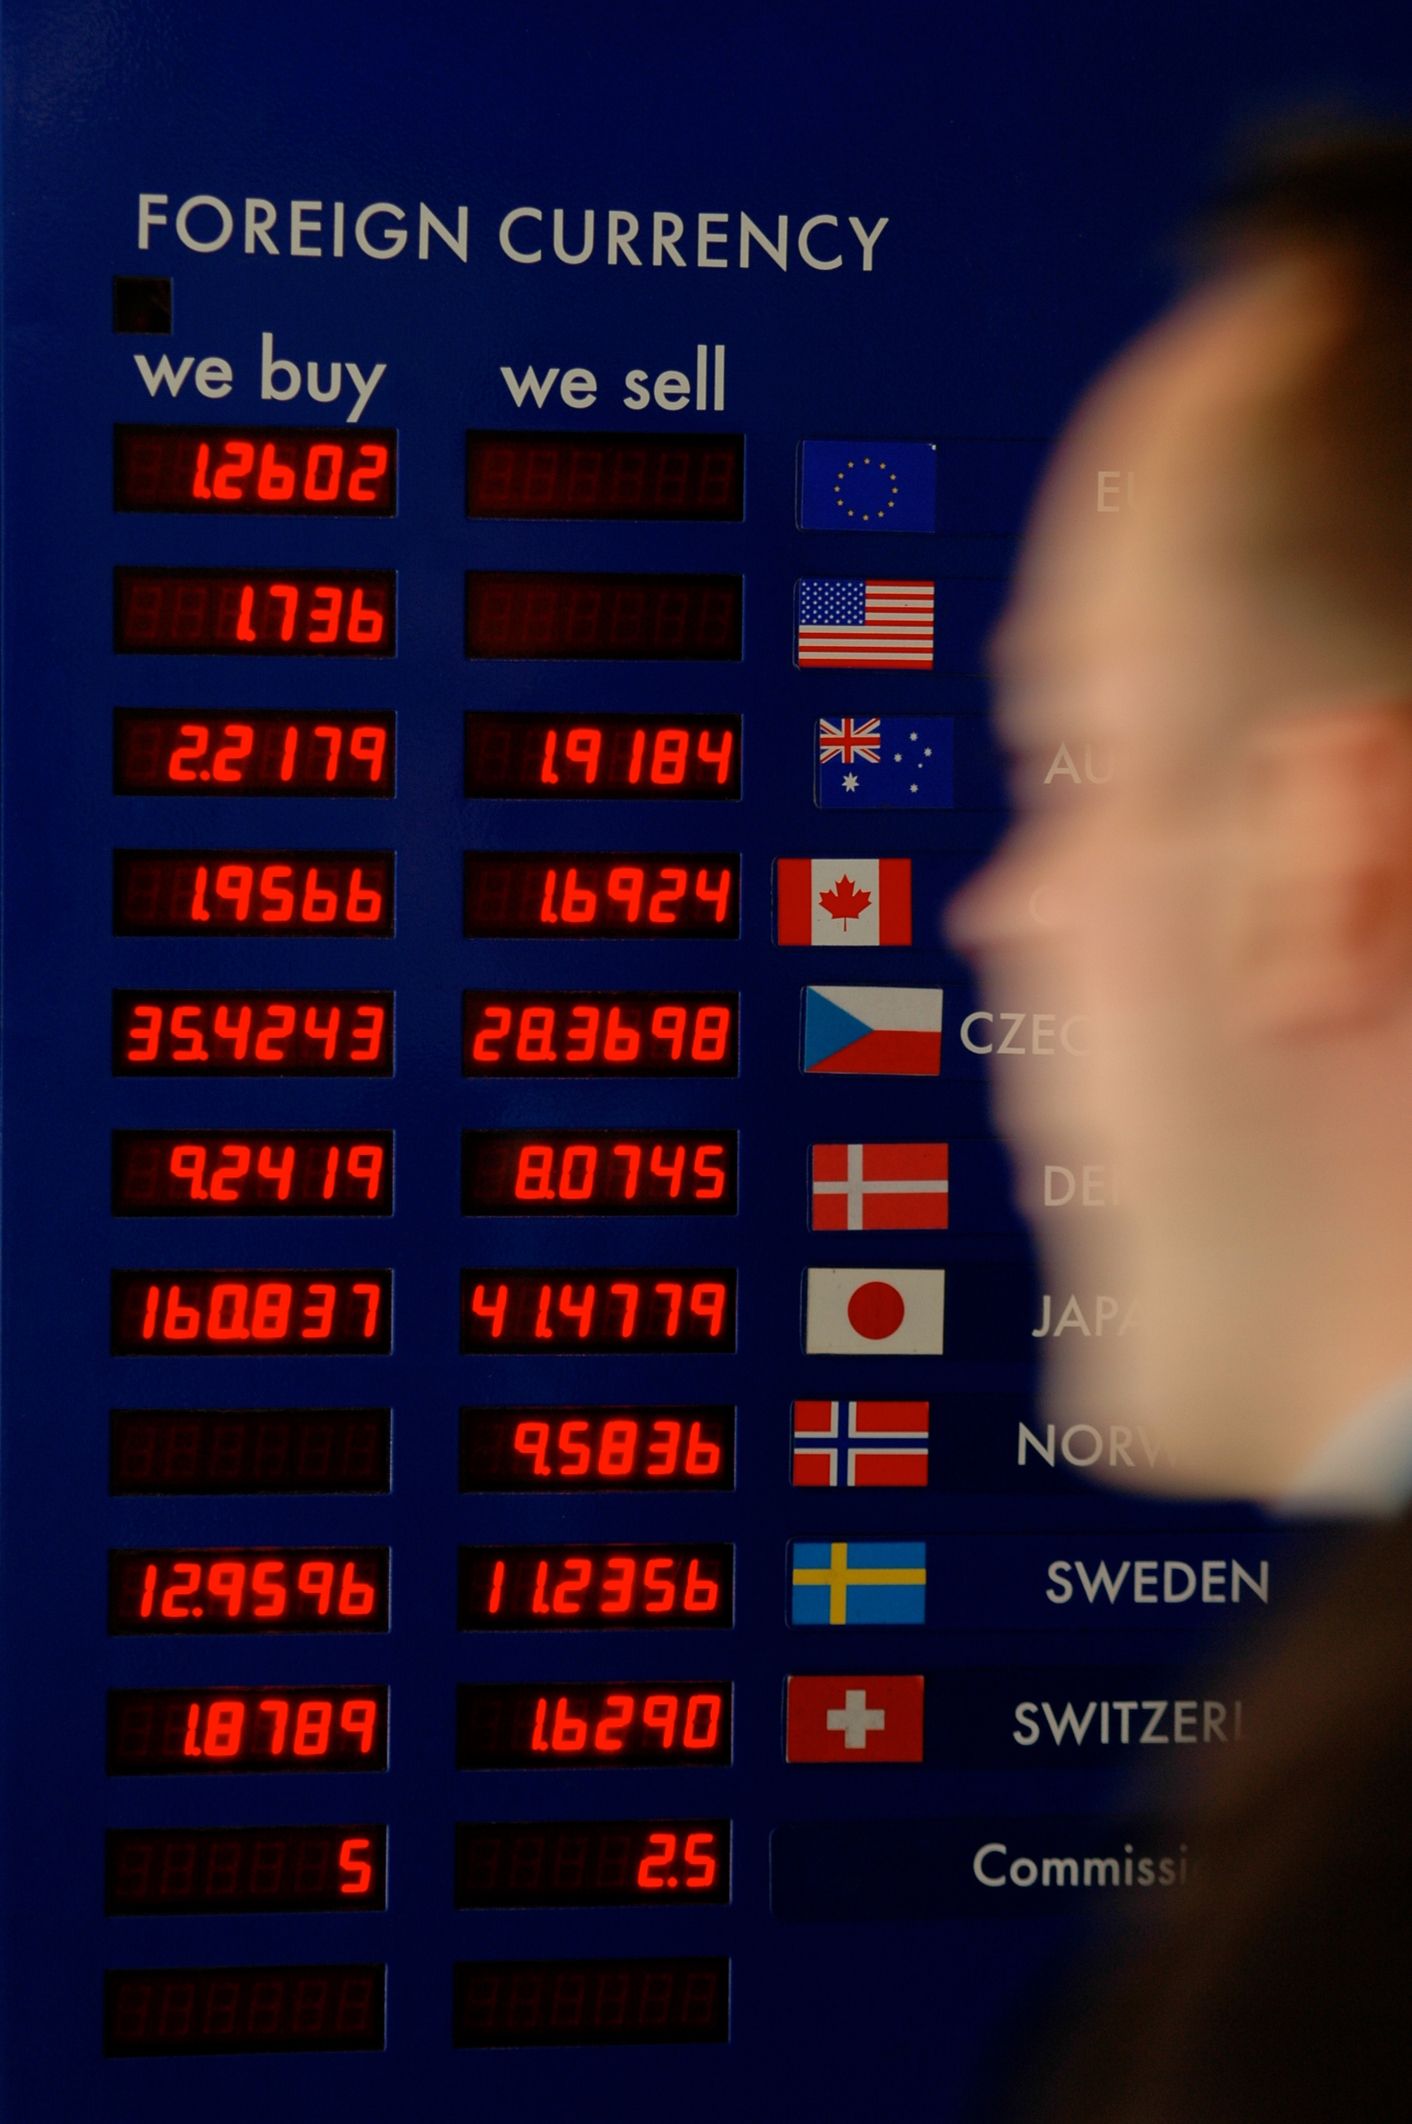
\includegraphics[width=.3\paperwidth]{pics/Image_XRates}
	\end{figure}
	\hyperlink{main2}{\beamerbutton{back}}
\end{frame}



\appendix

\begin{frame}<handout:0>[label=quote, noframenumbering]{Quote on fundamental value}
	John Maynard Keynes:
	``Certain classes of investment are governed by the average expectation of those who deal on the Stock Exchange as revealed in the price of shares, rather than by the genuine expectations of the professional entrepreneur.... 
	
	\quad
	
	In practice, we have tacitly agreed, as a rule, to fall back on what is, in truth, a convention. The essence of this convention -- though it does not, of course, work out so simply -- lies in assuming that the existing state of affairs will continue indefinitely, except in so far as we have specific reasons to expect a change.''
	\hyperlink{main4}{\beamerbutton{back}}
\end{frame}


\begin{frame}<handout:0>[label=LOB, noframenumbering]{Limit Order Book}
	\begin{figure}
	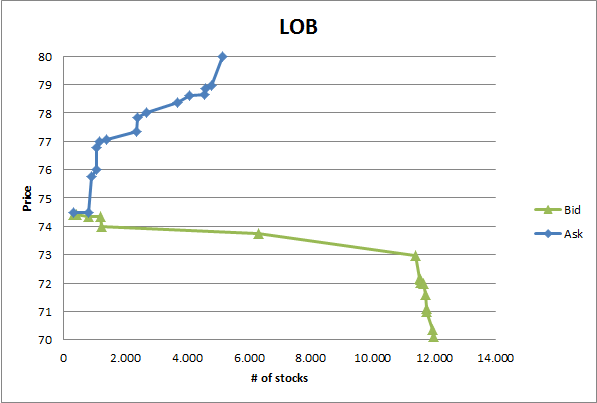
\includegraphics[width=.7\paperwidth]{pics/Graph_LOB}
	\end{figure}
	\hyperlink{main3}{\beamerbutton{back}}
\end{frame}

\end{document} 